


%🍁% \chapter{Inheritance}
\chapter{继承}

%🍁% The language feature most often associated with object-oriented
%🍁% programming is {\bf inheritance}.  Inheritance is the ability to
%🍁% define a new class that is a modified version of an existing class.
%🍁% In this chapter I demonstrate inheritance using classes that represent
%🍁% playing cards, decks of cards, and poker hands.

最常与面向对象编程联系在一起的语言特性就是 {\em 继承}。
继承指的是在现有类的基础下进行修改,从而定义新类的能力。
在本章中,我会用表示卡牌、一副牌和牌型的类\footnote{卡牌 (playing cards);一副牌
(deck of hands);牌型 (poker hands)。},来展示继承这一特性。

\index{deck}  \index{card, playing}  \index{poker}

%🍁% If you don't play
%🍁% poker, you can read about it at
%🍁% \url{http://en.wikipedia.org/wiki/Poker}, but you don't have to; I'll
%🍁% tell you what you need to know for the exercises.

如果你不玩扑克牌,你可以 \href{http://en.wikipedia.org/wiki/Poker}{阅读}了解一下,但这不是必须的;我会告诉你完成练习所需要了解的知识点。

%🍁% Code examples from
%🍁% this chapter are available from
%🍁% \url{http://thinkpython2.com/code/Card.py}.

%🍁% \section{Card objects}
\section{卡牌对象}

%🍁% There are fifty-two cards in a deck, each of which belongs to one of
%🍁% four suits and one of thirteen ranks.  The suits are Spades, Hearts,
%🍁% Diamonds, and Clubs (in descending order in bridge).  The ranks are
%🍁% Ace, 2, 3, 4, 5, 6, 7, 8, 9, 10, Jack, Queen, and King.  Depending on
%🍁% the game that you are playing, an Ace may be higher than King
%🍁% or lower than 2.

一副牌有52张牌,每一张属于4种花色的一个和13个等级的一个。
4种花色是黑桃、红心、方块、梅花 \footnote{黑桃 (Spades);红心 (Hearts);方块 (Diamonds);梅花 (Clubs)。},
以桥牌中的逆序排列。  13个等级是A、2、3、4、5、6、7、8、9、10、J、Q、K。
根据你玩的游戏的不同,A 可能比 K 大或者比 2 小。

\index{rank}  \index{suit}

%🍁% If we want to define a new object to represent a playing card, it is
%🍁% obvious what the attributes should be: {\tt rank} and
%🍁% {\tt suit}.  It is not as obvious what type the attributes
%🍁% should be.  One possibility is to use strings containing words like
%🍁% \verb"'Spade'" for suits and \verb"'Queen'" for ranks.  One problem with
%🍁% this implementation is that it would not be easy to compare cards to
%🍁% see which had a higher rank or suit.

如果我们定义一个新的对象来表示卡牌,明显它应该有 \li{rank} (等级) 和 \li{suit} (花色)
两个属性。  但两个属性的类型不太明显。  一个可能是使用字符串类型,
如 \li{'Spade'} 表示花色,\li{'Queen'} 表示等级。  这种实现的一个问题是,不是那么容易比较牌的大小,看哪张牌的等级或花色更高。

\index{encode}  \index{encrypt}
\index{map to}  \index{representation}

%🍁% An alternative is to use integers to {\bf encode} the ranks and suits.
%🍁% In this context, ``encode'' means that we are going to define a mapping
%🍁% between numbers and suits, or between numbers and ranks.  This
%🍁% kind of encoding is not meant to be a secret (that
%🍁% would be ``encryption'').

另外一种方法,是使用一个整型来 {\em 编码} 等级 和 花色。
在这里,``编码'' 表示我们要定义一个数字到花色或数字到等级的映射。
但是这里的编码并不是为了保密(那就成了``加密'')。

\newcommand{\mymapsto}{$\mapsto$}

%🍁% For example, this table shows the suits and the corresponding integer
%🍁% codes:

例如,下面的表格列出了花色和对应的整数码:

\begin{tabular}{l c l}
Spades & \mymapsto & 3 \\
Hearts & \mymapsto & 2 \\
Diamonds & \mymapsto & 1 \\
Clubs & \mymapsto & 0
\end{tabular}

%🍁% This code makes it easy to compare cards; because higher suits map to
%🍁% higher numbers, we can compare suits by comparing their codes.

整数码使得很容易比较牌的大小;因为更高的花色对应更高的数字,我们可以通过比较数字,来判断花色的的大小。

%🍁% The mapping for ranks is fairly obvious; each of the numerical ranks
%🍁% maps to the corresponding integer, and for face cards:

等级的映射类型选择就显而易见;每个数字等级对应相应的整数,然后对于J,K,Q:

\begin{tabular}{l c l}
Jack & \mymapsto & 11 \\
Queen & \mymapsto & 12 \\
King & \mymapsto & 13 \\
\end{tabular}

%🍁% I am using the \mymapsto~symbol to make it clear that these mappings
%🍁% are not part of the Python program.  They are part of the program
%🍁% design, but they don't appear explicitly in the code.

这里,我使用 \mymapsto~符号来清楚的表示,这些不是 Python 程序的一部分。  它们属于程序设计的一部分,但是不会出现在代码中。

\index{Card class}  \index{class!Card}

%🍁% The class definition for {\tt Card} looks like this:

\li{Card}类的定义如下:

\begin{lstlisting}
class Card:
    """Represents a standard playing card."""

    def __init__(self, suit=0, rank=2):
        self.suit = suit
        self.rank = rank
\end{lstlisting}

%
%🍁% As usual, the init method takes an optional
%🍁% parameter for each attribute.  The default card is
%🍁% the 2 of Clubs.

通常,init 方法接受针对每个属性的可选形参。默认的卡牌是梅花 2。

\index{init method}  \index{method!init}

%🍁% To create a Card, you call {\tt Card} with the
%🍁% suit and rank of the card you want.

可以使用你需要的花色和等级调用 \li{Card} ,创建一个 \li{Card} 对象。

\begin{lstlisting}
queen_of_diamonds = Card(1, 12)
\end{lstlisting}
%

%🍁% \section{Class attributes}
\section{类属性}

\label{class.attribute}
\index{class attribute}  \index{attribute!class}

%🍁% In order to print Card objects in a way that people can easily
%🍁% read, we need a mapping from the integer codes to the corresponding
%🍁% ranks and suits.  A natural way to
%🍁% do that is with lists of strings.  We assign these lists to {\bf class
%🍁% attributes}:

为了以大家能够轻松看懂的方式来打印卡牌对象,我们需要一个从整数码到对应的等级和花色的映射。
一种直接的方法是使用字符串列表。我们把这些列表赋值到 {\em 类属性} :

\begin{lstlisting}
# inside class Card:

    suit_names = ['Clubs', 'Diamonds', 'Hearts', 'Spades']
    rank_names = [None, 'Ace', '2', '3', '4', '5', '6', '7',
              '8', '9', '10', 'Jack', 'Queen', 'King']

    def __str__(self):
        return '%s of %s' % (Card.rank_names[self.rank],
                             Card.suit_names[self.suit])
\end{lstlisting}

%🍁% %
%🍁% Variables like \verb"suit_names" and \verb"rank_names", which are
%🍁% defined inside a class but outside of any method, are called
%🍁% class attributes because they are associated with the class object
%🍁% {\tt Card}.

像 \li{suit_names} 和 \li{rank_names} 这样的变量,是定义在类内部但在方法之外,
被称为类属性。因为他们是被关联到 \li{Card} 类对象上的。

\index{instance attribute}  \index{attribute!instance}

%🍁% This term distinguishes them from variables like {\tt suit} and {\tt
%🍁%   rank}, which are called {\bf instance attributes} because they are
%🍁% associated with a particular instance.
%🍁% \index{dot notation}

这个术语将它们同 \li{suit} 和 \li{rank} 这样的变量区分开来,后者被称为 {\em 实例属性},
因为他们被关联到了特定的实例。

%🍁% Both kinds of attribute are accessed using dot notation.  For
%🍁% example, in \verb"__str__", {\tt self} is a Card object,
%🍁% and {\tt self.rank} is its rank.  Similarly, {\tt Card}
%🍁% is a class object, and \verb"Card.rank_names" is a
%🍁% list of strings associated with the class.

这两种属性都使用点标记法来访问。
例如,在 \li{__str__} 中, \li{self} 是一个卡牌对象, \li{self.rank} 是它的等级。
同样的, \li{Card} 是一个类对象, \li{Card.rank_names} 是一个和类关联的字符串列表。

%🍁% Every card has its own {\tt suit} and {\tt rank}, but there
%🍁% is only one copy of \verb"suit_names" and \verb"rank_names".

每一张卡牌都有自己的花色和等级,
但是这里只有一份 \li{suit_names} 和 \li{rank_names} 拷贝。

%🍁% Putting it all together, the expression
%🍁% \verb"Card.rank_names[self.rank]" means ``use the attribute {\tt rank}
%🍁% from the object {\tt self} as an index into the list \verb"rank_names"
%🍁% from the class {\tt Card}, and select the appropriate string.''

综合来说,表达式 \li{Card.rank_names[self.rank]} 表示 ``使用 \li{self} 对象
中的 \li{rank} 属性作为 \li{Card} 类的 \li{rank_names}
列表的索引下标,然后获取相应的字符串。''

%🍁% The first element of \verb"rank_names" is {\tt None} because there
%🍁% is no card with rank zero.  By including {\tt None} as a place-keeper,
%🍁% we get a mapping with the nice property that the index 2 maps to the
%🍁% string \verb"'2'", and so on.  To avoid this tweak, we could have
%🍁% used a dictionary instead of a list.

\li{rank_names} 的第一个元素是 \li{None} ,因为没有卡牌的等级是 0 。
通过使用 \li{None} 作为占位符,我们可以很好地将索引 2 映射到字符串 \li{'2'} ,等等。
为了避免使用这种小技巧,我们也可以使用一个字典来代替列表。

%🍁% With the methods we have so far, we can create and print cards:

利用现有的方法,我们可以创建和打印卡牌:

\begin{lstlisting}
>>> card1 = Card(2, 11)
>>> print(card1)
Jack of Hearts
\end{lstlisting}

\begin{figure}
\centerline
{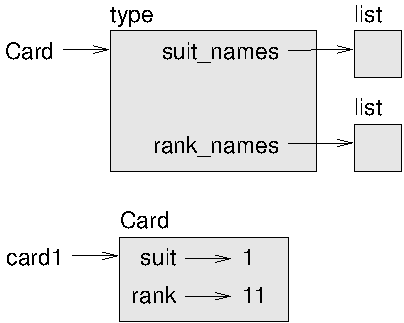
\includegraphics[scale=0.8]{../source/figs/card1.pdf}}
%🍁% \caption{Object diagram.}
\caption{对象图。}
\label{fig.card1}
\end{figure}

%🍁% Figure~\ref{fig.card1} is a diagram of the {\tt Card} class object and
%🍁% one Card instance.  {\tt Card} is a class object; its type is {\tt
%🍁%   type}.  {\tt card1} is an instance of {\tt Card}, so its type is
%🍁% {\tt Card}.  To save space, I didn't draw the contents of
%🍁% \verb"suit_names" and \verb"rank_names".

图~\ref{fig.card1} 是 \li{Card} 类对象和一个 \li{Card} 实例的图示。 \li{Card} 是一个类对象;它的类型是 \li{type} 。 \li{card1} 是 \li{Card} 的一个实例,因此它的类型是 \li{Card}。 为了节省空间,我没有画出 \li{suit_names} 和 \li{rank_names} 的内容。

\index{state diagram}  \index{diagram!state}
\index{object diagram}  \index{diagram!object}


%🍁% \section{Comparing cards}
\section{卡牌比较}

\label{comparecard}
\index{operator!relational}
\index{relational operator}

%🍁% For built-in types, there are relational operators
%🍁% ({\tt <}, {\tt >}, {\tt ==}, etc.)
%🍁% that compare
%🍁% values and determine when one is greater than, less than, or equal to
%🍁% another.  For programmer-defined types, we can override the behavior of
%🍁% the built-in operators by providing a method named
%🍁% \verb"__lt__", which stands for ``less than''.

对于内建类型,有关系运算符(<, >, ==, 等等)可以比较值,判断哪一个是大于、小于或等于另外一个。
对于程序员自定义的类型,我们可以通过提供一个叫 \li{__lt__} (代表“小于”)的方法,来覆盖内建运算符的行为。

\index{programmer-defined type}
\index{type!programmer-defined}

%🍁% \verb"__lt__" takes two parameters, {\tt self} and {\tt other},
%🍁% and {\tt True} if {\tt self} is strictly less than {\tt other}.

\li{__lt__} 接受 2 个参数, \li{self} 和 \li{other},如果 \li{self} 比 \li{other} 的值要小则返回 \li{True} 。

\index{override}
\index{operator overloading}

%🍁% The correct ordering for cards is not obvious.
%🍁% For example, which
%🍁% is better, the 3 of Clubs or the 2 of Diamonds?  One has a higher
%🍁% rank, but the other has a higher suit.  In order to compare
%🍁% cards, you have to decide whether rank or suit is more important.

卡牌的正确顺序并不明显。
例如,梅花 3 和方块 2 哪个更高?
一个等级更高,另一个花色更高。
为了比较卡牌,你必须决定等级还是花色更重要。

%🍁% The answer might depend on what game you are playing, but to keep
%🍁% things simple, we'll make the arbitrary choice that suit is more
%🍁% important, so all of the Spades outrank all of the Diamonds,
%🍁% and so on.

答案可能根据你玩的是什么游戏而不同,但是简洁起见,
我们将规定花色更重要,所以所有的黑桃大于任何方块卡牌,以此类推。

\index{cmp method@\_\_cmp\_\_ method}
\index{method!\_\_cmp\_\_}

%🍁% With that decided, we can write \verb"__lt__":

定好了这个规则后,我们可以编写 \li{__lt__} 了:

\begin{lstlisting}
# inside class Card:
# 在Card类内部:

    def __lt__(self, other):
        # check the suits
        # 判断花色
        if self.suit < other.suit: return True
        if self.suit > other.suit: return False

        # suits are the same... check ranks
        # 花色相同...判断等级
        return self.rank < other.rank
\end{lstlisting}

%🍁% %
%🍁% You can write this more concisely using tuple comparison:

你可以使用元组比较来使得代码更加简洁:

\index{tuple!comparison}
\index{comparison!tuple}

\begin{lstlisting}
# inside class Card:

    def __lt__(self, other):
        t1 = self.suit, self.rank
        t2 = other.suit, other.rank
        return t1 < t2
\end{lstlisting}

%
%🍁% As an exercise, write an \verb"__lt__" method for Time objects.  You
%🍁% can use tuple comparison, but you also might consider
%🍁% comparing integers.

我们做个练习,编写一个 \li{Time} 对象的 \li{__lt__}方法。
你可以使用元组比较,也可以考虑比较整数。


%🍁% \section{Decks}
\section{一副牌}

\index{list!of objects}
\index{deck, playing cards}

%🍁% Now that we have Cards, the next step is to define Decks.  Since a
%🍁% deck is made up of cards, it is natural for each Deck to contain a
%🍁% list of cards as an attribute.

现在我们有 \li{Card} 类了,下一步是定义完整的一副牌 (Deck)了。
因为一副牌由许多牌组成,自然地每一个 \li{Deck} 都有一个卡牌列表作为属性。

\index{init method}
\index{method!init}

%🍁% The following is a class definition for {\tt Deck}.  The
%🍁% init method creates the attribute {\tt cards} and generates
%🍁% the standard set of fifty-two cards:

下面是一个 \li{Deck} 的类定义。
初始化方法创建了 \li{cards} 属性, 然后生成了由 52 张牌组成一副标准卡牌。

\index{composition}  \index{loop!nested}
\index{Deck class}  \index{class!Deck}

\begin{lstlisting}
class Deck:

    def __init__(self):
        self.cards = []
        for suit in range(4):
            for rank in range(1, 14):
                card = Card(suit, rank)
                self.cards.append(card)
\end{lstlisting}

%🍁% %
%🍁% The easiest way to populate the deck is with a nested loop.  The outer
%🍁% loop enumerates the suits from 0 to 3.  The inner loop enumerates the
%🍁% ranks from 1 to 13.  Each iteration
%🍁% creates a new Card with the current suit and rank,
%🍁% and appends it to {\tt self.cards}.

生成一副牌的最简单方法是使用嵌套循环。
外层循环枚举 0 到 3 的花色。
内层循环枚举 1 到 13 的等级。
每一个迭代都用当前的花色和等级创建一张新的牌。
然后放入 \li{self.cards} 中。

\index{append method}
\index{method!append}


%🍁% \section{Printing the deck}
\section{打印一副牌}

\label{printdeck}
\index{str method@\_\_str\_\_ method}
\index{method!\_\_str\_\_}

%🍁% Here is a \verb"__str__" method for {\tt Deck}:

下面是为 \li{Deck} 定义的 \li{__str__} 方法:

\begin{lstlisting}
#inside class Deck:

    def __str__(self):
        res = []
        for card in self.cards:
            res.append(str(card))
        return '\n'.join(res)
\end{lstlisting}

%
%🍁% This method demonstrates an efficient way to accumulate a large
%🍁% string: building a list of strings and then using the string method
%🍁% {\tt join}.  The built-in function {\tt str} invokes the
%🍁% \verb"__str__" method on each card and returns the string
%🍁% representation.

这个方法展示了累积大字符串的高效方法:建立一个字符串列表然后使用字符串方法 \li{join}。
内建函数 \li{str} 会调用每个卡牌上的 \li{__str__} 方法,并返回它们的字符串表示。

\index{accumulator!string} \index{string!accumulator}
\index{join method} \index{method!join} \index{newline}

%🍁% Since we invoke {\tt join} on a newline character, the cards
%🍁% are separated by newlines.  Here's what the result looks like:

由于我们是在一个换行符上调用的 \li{join} ,卡牌之间被换行符分隔。  下面是结果示例:

\begin{lstlisting}
>>> deck = Deck()
>>> print(deck)
Ace of Clubs
2 of Clubs
3 of Clubs
...
10 of Spades
Jack of Spades
Queen of Spades
King of Spades
\end{lstlisting}

%
%🍁% Even though the result appears on 52 lines, it is
%🍁% one long string that contains newlines.

虽然这个结果有52行,但他实际上是包含换行符的一个长字符串。

%🍁% \section{Add, remove, shuffle and sort}
\section{添加,移除,洗牌和排序}

%🍁% To deal cards, we would like a method that
%🍁% removes a card from the deck and returns it.
%🍁% The list method {\tt pop} provides a convenient way to do that:

为了发牌,我们需要一个可以把卡牌从一副牌中移除并返回的方法。
列表的 \li{pop} 方法提供了一个便捷的实现:

\index{pop method}
\index{method!pop}

\begin{lstlisting}
#inside class Deck:

    def pop_card(self):
        return self.cards.pop()
\end{lstlisting}

%🍁% %
%🍁% Since {\tt pop} removes the {\em last} card in the list, we are
%🍁% dealing from the bottom of the deck.

由于 \li{pop} 移除列表的 {\bf 最后一张} 卡牌,所以我们从牌底开始发牌。

\index{append method}
\index{method!append}

%🍁% To add a card, we can use the list method {\tt append}:

\begin{lstlisting}
#inside class Deck:

    def add_card(self, card):
        self.cards.append(card)
\end{lstlisting}

%🍁% %
%🍁% A method like this that uses another method without doing
%🍁% much work is sometimes called a {\bf veneer}.  The metaphor
%🍁% comes from woodworking, where a veneer is a thin
%🍁% layer of good quality wood glued to the surface of a cheaper piece of
%🍁% wood to improve the appearance.

像上面这样利用别的方法 (method),自己却没有做太多处理的方法,
有时候被称为 {\em 伪装方法} (veneer)。
这个隐喻来源于木工行业, 他们通常用一片高质量的木质薄层粘贴在一块便宜木材的表面,改善外观形象。

\index{veneer}

%🍁% In this case \verb"add_card" is a ``thin'' method that expresses
%🍁% a list operation in terms appropriate for decks.  It
%🍁% improves the appearance, or interface, of the
%🍁% implementation.

在这里,\li{add_card} 是一个 ``瘦'' 方法,以卡牌的术语来表述一个列表操作。
它改善了实现的外观,或者说接口。

%🍁% As another example, we can write a Deck method named {\tt shuffle}
%🍁% using the function {\tt shuffle} from the {\tt random} module:

再举一个例子,我们可以用 \li{random} 模块中的
\li{shuffle} 函数,给 \li{Deck} 写一个叫 \li{shuffle} 的方法。

\index{random module}
\index{module!random}
\index{shuffle function}
\index{function!shuffle}

\begin{lstlisting}
# inside class Deck:

    def shuffle(self):
        random.shuffle(self.cards)
\end{lstlisting}

%🍁% %
%🍁% Don't forget to import {\tt random}.

不要忘记了导入 \li{random} 。

%🍁% As an exercise, write a Deck method named {\tt sort} that uses the
%🍁% list method {\tt sort} to sort the cards in a {\tt Deck}.  {\tt sort}
%🍁% uses the \verb"__lt__" method we defined to determine the order.

我们做个练习,用列表的 \li{sort} 方法来写一个 \li{Deck} 的 \li{sort} 方法,给卡牌排序。
 \li{sort} 使用我们定义的 \li{__cmp__} 来决定排序顺序。

\index{sort method} \index{method!sort}


%🍁% \section{Inheritance}
\section{继承}

\index{inheritance}
\index{object-oriented programming}

%🍁% Inheritance is the ability to define a new class that is a modified
%🍁% version of an existing class.  As an example, let's say we want a
%🍁% class to represent a ``hand'', that is, the cards held by one player.
%🍁% A hand is similar to a deck: both are made up of a collection of
%🍁% cards, and both require operations like adding and removing cards.

继承指的是在现有类的基础下进行修改,从而定义新类的能力。
例如,假设我们想定义一个类来代表手牌 (hand) ,即玩家目前手里有的牌。
手牌与一副牌 (deck)类似:二者都由卡牌组成,都要求支持添加和移除卡牌的操作。

%🍁% A hand is also different from a deck; there are operations we want for
%🍁% hands that don't make sense for a deck.  For example, in poker we
%🍁% might compare two hands to see which one wins.  In bridge, we might
%🍁% compute a score for a hand in order to make a bid.

但二者也有区别;有些我们希望手牌具备的操作,对于 deck 来说并不合理。
例如,在扑克牌中,我们可能需要比较两个手牌,比较哪方赢了。
在桥牌中,我们可能需要计算手牌的得分,才好下注。

%🍁% This relationship between classes---similar, but different---lends
%🍁% itself to inheritance.
%🍁% To define a new class that inherits from an existing class,
%🍁% you put the name of the existing class in parentheses:

类之间有相似之处,但也存在不同,这时就可以用上继承了。
你只需要在定义新类时,将现有类的名称放在括号里,即可继承现有类:

\index{parentheses!parent class in}
\index{parent class}
\index{class!parent}
\index{Hand class}
\index{class!Hand}

\begin{lstlisting}
class Hand(Deck):
    """Represents a hand of playing cards."""
\end{lstlisting}

%🍁% %
%🍁% This definition indicates that {\tt Hand} inherits from {\tt Deck};
%🍁% that means we can use methods like \verb"pop_card" and \verb"add_card"
%🍁% for Hands as well as Decks.

这个定义表明,\li{Hand} 继承自 \li{Deck} ;  这意味着我们也可以对 \li{Hands} 使用 \li{Deck} 的 \li{pop_card} 和 \li{add_card} 方法。

%🍁% When a new class inherits from an existing one, the existing
%🍁% one is called the {\bf parent} and the new class is
%🍁% called the {\bf child}.

当一个新类继承自一个现有类时,现有类被称为 {\em 父类} (parent) ,新类被称为 {\em 子类} (child) 。

\index{parent class}
\index{child class}
\index{class!child}

%🍁% In this example, {\tt Hand} inherits \verb"__init__" from {\tt Deck},
%🍁% but it doesn't really do what we want: instead of populating the hand
%🍁% with 52 new cards, the init method for Hands should initialize {\tt
%🍁%   cards} with an empty list.  \index{override} \index{init method}

在此例中, \li{Hand} 继承了 \li{Deck} 的 \li{__init__} 方法,
但是它并没有满足我们的要求:init 方法应该为 \li{Hand} 初始化一个空的 \li{cards}
列表,而不是往手牌里添加 52 张新牌。

\index{method!init}

%🍁% If we provide an init method in the {\tt Hand} class, it overrides the
%🍁% one in the {\tt Deck} class:

如果我们提供一个 \li{Hand} 的 init 方法,它会覆盖从 \li{Deck} 类继承来的同名方法。

\begin{lstlisting}
# inside class Hand:

    def __init__(self, label=''):
        self.cards = []
        self.label = label
\end{lstlisting}

%🍁% %
%🍁% When you create a Hand, Python invokes this init method, not the
%🍁% one in {\tt Deck}.

当你创建一个 \li{Hand} 时,Python 会调用这个 init 方法,而不是 \li{Deck} 中的同名方法。

\begin{lstlisting}
>>> hand = Hand('new hand')
>>> hand.cards
[]
>>> hand.label
'new hand'
\end{lstlisting}

%🍁% %
%🍁% The other methods are inherited from {\tt Deck}, so we can use
%🍁% \verb"pop_card" and \verb"add_card" to deal a card:

其它方法是从 \li{Deck} 继承来的,所以我们可以使用 \li{pop_card} 和
\li{add_card} 来发牌:

\begin{lstlisting}
>>> deck = Deck()
>>> card = deck.pop_card()
>>> hand.add_card(card)
>>> print(hand)
King of Spades
\end{lstlisting}

%🍁% %
%🍁% A natural next step is to encapsulate this code in a method
%🍁% called \verb"move_cards":

很自然地,下一步就是把这些代码封装进一个叫 \li{move_cards} 的方法:

\index{encapsulation}

\begin{lstlisting}
#inside class Deck:

    def move_cards(self, hand, num):
        for i in range(num):
            hand.add_card(self.pop_card())
\end{lstlisting}

%🍁% %
%🍁% \verb"move_cards" takes two arguments, a Hand object and the number of
%🍁% cards to deal.  It modifies both {\tt self} and {\tt hand}, and
%🍁% returns {\tt None}.

\li{move_cards} 接受两个参数,一个是 \li{Hand} 对象,另一个是发牌的数量。
它会同时修改 \li{self} 和 \li{hand} ,然后返回 \li{None} 。

%🍁% In some games, cards are moved from one hand to another,
%🍁% or from a hand back to the deck.  You can use \verb"move_cards"
%🍁% for any of these operations: {\tt self} can be either a Deck
%🍁% or a Hand, and {\tt hand}, despite the name, can also be a {\tt Deck}.

在有些游戏里面,卡牌从一个手牌移动到另外一个手牌,或者从手牌退还到牌堆里面。
任何这些操作都可以使用 \li{move_cards} : \li{self} 可以是一个 \li{Deck} 或者一个 \li{Hand} ,而且尽管名字叫 \li{hand} ,它也可以是一个 \li{Deck} 。

%🍁% Inheritance is a useful feature.  Some programs that would be
%🍁% repetitive without inheritance can be written more elegantly
%🍁% with it.  Inheritance can facilitate code reuse, since you can
%🍁% customize the behavior of parent classes without having to modify
%🍁% them.  In some cases, the inheritance structure reflects the natural
%🍁% structure of the problem, which makes the design easier to
%🍁% understand.

继承是一个非常有用的特性。有了继承,一些重复性的代码可以写得非常的优雅。
继承有助于代码重用,因为你可以在不修改父类定义的前提下,就改变父类的行为。
在有些情况下,继承的结构反映了真实问题的结构,使得程序更易于理解。

%🍁% On the other hand, inheritance can make programs difficult to read.
%🍁% When a method is invoked, it is sometimes not clear where to find its
%🍁% definition.  The relevant code may be spread across several modules.
%🍁% Also, many of the things that can be done using inheritance can be
%🍁% done as well or better without it.

另一方面,继承又有可能会使得程序更加难读。
当调用一个方法时,有时候搞不清楚去哪找它的定义。
相关的代码可能被分散在几个模块之中。
而且,许多用继承能完成的事情,不用继承也可以完成,有可能还完成得更好。

%🍁% \section{Class diagrams}
\section{类图}
\label{class.diagram}

%🍁% So far we have seen stack diagrams, which show the state of
%🍁% a program, and object diagrams, which show the attributes
%🍁% of an object and their values.  These diagrams represent a snapshot
%🍁% in the execution of a program, so they change as the program
%🍁% runs.

到目前为止我们已经了解过栈图,它显示的是一个程序的状态;
以及对象图,它显示的是一个对象的属性及其值。
这些图代表了程序执行中的一个快照,所以它们随着程序的运行而变化。

%🍁% They are also highly detailed; for some purposes, too
%🍁% detailed.  A class diagram is a more abstract representation
%🍁% of the structure of a program.  Instead of showing individual
%🍁% objects, it shows classes and the relationships between them.

它们也十分的详细;但有些时候显得过于详细了。
类图是程序结构的一种更加抽象的表达。
它显示的是类和类之间的关系,而不是每个独立的对象。

%🍁% There are several kinds of relationship between classes:

类之间有如下几种关系:

\begin{itemize}

%🍁% \item Objects in one class might contain references to objects
%🍁% in another class.  For example, each Rectangle contains a reference
%🍁% to a Point, and each Deck contains references to many Cards.
%🍁% This kind of relationship is called {\bf HAS-A}, as in, ``a Rectangle
%🍁% has a Point.''

\item 一个类中的对象可以包含对另外一个类的对象的引用。
例如,每一个矩形包含对点的引用,每一个 \li{Deck} 包含对许多 \li{Card} 的引用。 这种关系被称为{\em 组合} ({\bf HAS-A}),可以类似这样描述:``一个矩形有一个点\footnote{``a Rectangle has a Point.''}''。

%🍁% \item One class might inherit from another.  This relationship
%🍁% is called {\bf IS-A}, as in, ``a Hand is a kind of a Deck.''

\item 一个类可能继承自另外一个类。
这种关系被称为 {\em 继承} ({\bf IS-A}), 可以类似这样描述:``Hand is a kind of Deck''。

%🍁% \item One class might depend on another in the sense that objects
%🍁% in one class take objects in the second class as parameters, or
%🍁% use objects in the second class as part of a computation.  This
%🍁% kind of relationship is called a {\bf dependency}.

\item 一个类可能强赖另一个类,因为前者中的对象接受后者中的对象作为参数,
或者使用后者中的对象作为计算的一部分。这种关系被称为 {\em 依赖} ({\bf dependency})。

\end{itemize}

\index{IS-A relationship}
\index{HAS-A relationship}
\index{class diagram}
\index{diagram!class}

%🍁% A {\bf class diagram} is a graphical representation of these
%🍁% relationships.  For example, Figure~\ref{fig.class1} shows the
%🍁% relationships between {\tt Card}, {\tt Deck} and {\tt Hand}.

类图是这些关系的图形化表示。  例如,图~\ref{fig.class1} 标明了 \li{Card} , \li{Deck} 和
\li{Hand} 之间的关系。

\begin{figure}
\centerline
{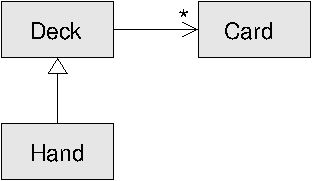
\includegraphics[scale=0.8]{../source/figs/class1.pdf}}
%🍁% \caption{Class diagram.}
\caption{类图。}
\label{fig.class1}
\end{figure}

%🍁% The arrow with a hollow triangle head represents an IS-A
%🍁% relationship; in this case it indicates that Hand inherits
%🍁% from Deck.

带空心三角的箭头表示 IS-A 的关系; 这里它表示 \li{Hand} 继承自 \li{Deck} 。

%🍁% The standard arrow head represents a HAS-A
%🍁% relationship; in this case a Deck has references to Card
%🍁% objects.

标准箭头表示 HAS-A 的关系; 这里表示 \li{Deck} 包含对 \li{Card} 对象的引用。

\index{multiplicity (in class diagram)}

%🍁% The star ({\tt *}) near the arrow head is a
%🍁% {\bf multiplicity}; it indicates how many Cards a Deck has.
%🍁% A multiplicity can be a simple number, like {\tt 52}, a range,
%🍁% like {\tt 5..7} or a star, which indicates that a Deck can
%🍁% have any number of Cards.

箭头旁边的星号是一个复数 ({\bf multiplicity})表达;
它表示 \li{Deck} 包含多少个 \li{Card}。
一个复数表达可以是一个简单的数字(如 52 ),
一个范围(如 \li{5..7} 或者是 \li{*},表示有任意数量的 \li{Card} 。

%🍁% There are no dependencies in this diagram.  They would normally
%🍁% be shown with a dashed arrow.  Or if there are a lot of
%🍁% dependencies, they are sometimes omitted.

图中没有标出依赖关系。  这种关系通常使用虚线箭头表示。
或者,如果有很多依赖关系的话,有时候会省略。

%🍁% A more detailed diagram might show that a Deck actually
%🍁% contains a {\em list} of Cards, but built-in types
%🍁% like list and dict are usually not included in class diagrams.

一个更详细的类图可能会显示 \li{Deck} 实际包含了一个由 \li{Cards} 组成的列表,但是通常类图中不会包含 \li{list} 和 \li{dict} 等内建类型。


%🍁% \section{Data encapsulation}
\section{数据封装}

%🍁% The previous chapters demonstrate a development plan we might call
%🍁% ``object-oriented design''.  We identified objects we needed---like
%🍁% {\tt Point}, {\tt Rectangle} and {\tt Time}---and defined classes to
%🍁% represent them.  In each case there is an obvious correspondence
%🍁% between the object and some entity in the real world (or at least a
%🍁% mathematical world).

前面几章中描述了一种可以称为 ``面向对象设计'' 的开发计划。
我们确定所需要的对象 --- 如 \li{Point}、 \li{Rectangle} 和 \li{Time} --- 然后定义代表它们的类。
对于每个类来说,这个类对象和真实世界(或至少是数学世界)中的某种实体具有明显的对应关系。

\index{development plan!data encapsulation}

%🍁% But sometimes it is less obvious what objects you need
%🍁% and how they should interact.  In that case you need a different
%🍁% development plan.  In the same way that we discovered function
%🍁% interfaces by encapsulation and generalization, we can discover
%🍁% class interfaces by {\bf data encapsulation}.

但是有时有很难界定你需要的对象以及它们如何交互。
在这个时候, 你需要一个不同的开发计划。
之前我们通过封装和泛化来编写函数接口, 我们同样可以通过 {\em 数据封装} 来编写类接口。

\index{data encapsulation}

%🍁% Markov analysis, from Section~\ref{markov}, provides a good example.
%🍁% If you download my code from \url{http://thinkpython2.com/code/markov.py},
%🍁% you'll see that it uses two global variables---\verb"suffix_map" and
%🍁% \verb"prefix"---that are read and written from several functions.

\ref{markov}~节 中介绍的马尔科夫分析就是一个很好的例子。
如果你下载我的\href{http://thinkpython2.com/code/markov.py}{代码}, 你会发现它使用了两个全局变量 —— \li{suffix_map} 和 \li{prefix}, 它们被多个函数进行读写。

\begin{lstlisting}
suffix_map = {}
prefix = ()
\end{lstlisting}

%🍁% Because these variables are global, we can only run one analysis at a
%🍁% time.  If we read two texts, their prefixes and suffixes would be
%🍁% added to the same data structures (which makes for some interesting
%🍁% generated text).

因为这些变量是全局的,我们一次只能运行一个分析。如果我们读取了两个文本,
它们的前缀和后缀会被加入相同的数据结构(会使得输出文本混乱)。

%🍁% To run multiple analyses, and keep them separate, we can encapsulate
%🍁% the state of each analysis in an object.
%🍁% Here's what that looks like:

如果想同时运行多个分析,并且保持它们的相互独立,我们可以把每个分析的状态封装到一个对象中。
下面是一个示例:

\begin{lstlisting}
class Markov:

    def __init__(self):
        self.suffix_map = {}
        self.prefix = ()
\end{lstlisting}

%🍁% Next, we transform the functions into methods.  For example,
%🍁% here's \verb"process_word":

下一步,我们把这些函数转换为方法。
例如:下面是 \li{process_word} :

\begin{lstlisting}
    def process_word(self, word, order=2):
        if len(self.prefix) < order:
            self.prefix += (word,)
            return

        try:
            self.suffix_map[self.prefix].append(word)
        except KeyError:
            # if there is no entry for this prefix, make one
            self.suffix_map[self.prefix] = [word]

        self.prefix = shift(self.prefix, word)
\end{lstlisting}

%🍁% Transforming a program like this---changing the design without
%🍁% changing the behavior---is another example of refactoring
%🍁% (see Section~\ref{refactoring}).

像这样改变一个程序 --- 改变设计而保持功能不变 --- 是代码重构的另一个例子
(参见\ref{refactoring}~节)。

\index{refactoring}

%🍁% This example suggests a development plan for designing objects and
%🍁% methods:

下面的例子给出了一种设计对象和方法的开发计划:

\begin{enumerate}

%🍁% \item Start by writing functions that read and write global
%🍁% variables (when necessary).
%🍁%
%🍁% \item Once you get the program working, look for associations
%🍁% between global variables and the functions that use them.
%🍁%
%🍁% \item Encapsulate related variables as attributes of an object.
%🍁%
%🍁% \item Transform the associated functions into methods of the new
%🍁% class.

\item 首先编写读取全局变量的函数(如有必要)。

\item 一旦你让程序跑起来了,开始查找全局变量和使用它们的函数的联系。

\item 封装相关的变量作为一个对象的属性。

\item 转换相关函数为新类的方法。

\end{enumerate}

%🍁% As an exercise, download my Markov code from
%🍁% \url{http://thinkpython2.com/code/markov.py}, and follow the steps
%🍁% described above to encapsulate the global variables as attributes of a
%🍁% new class called {\tt Markov}.  Solution:
%🍁% \url{http://thinkpython2.com/code/Markov.py} (note the capital M).

我们做个练习,下载我的\href{http://thinkpython2.com/code/markov.py}{马尔科夫分析代码},然后按照上面所述的步骤,将全局变量封装为新类 \li{Markov} (注意M为大写)的属性。


%🍁% \section{Debugging}
\section{调试}
\index{debugging}

%🍁% Inheritance can make debugging difficult because when you invoke a
%🍁% method on an object, it might be hard to figure out which method will
%🍁% be invoked.

继承会使得调试变得更加复杂,因为你可能不知道实际调用的是哪个类的方法。

\index{inheritance}

%🍁% Suppose you are writing a function that works with Hand objects.
%🍁% You would like it to work with all kinds of Hands, like
%🍁% PokerHands, BridgeHands, etc.  If you invoke a method like
%🍁% {\tt shuffle}, you might get the one defined in {\tt Deck},
%🍁% but if any of the subclasses override this method, you'll
%🍁% get that version instead.  This behavior is usually a good
%🍁% thing, but it can be confusing.

假设你在写一个处理 \li{Hand} 对象的函数。
你可能会想让它可以处理所有种类的 \li{Hand} ,
如 \li{PockerHands} , \li{BridgeHands} ,等等。
如果你调用类似 \li{shuffle} 这样的方法,你可能会得到 \li{Deck} 中定义的那个,
但是如果有任何一个子类覆盖了这个方法。你实际上得到的是子类的那个方法。
这个行为通常是一件好事,但是容易让人混淆。

%🍁% Any time you are unsure about the flow of execution through your
%🍁% program, the simplest solution is to add print statements at the
%🍁% beginning of the relevant methods.  If {\tt Deck.shuffle} prints a
%🍁% message that says something like {\tt Running Deck.shuffle}, then as
%🍁% the program runs it traces the flow of execution.

只要你不确定程序的执行流程,最简单的方法是在相关方法的开始处添加 \li{print} 语
句。  如果 \li{Deck.shuffle} 打印一条如像 \li{Running Deck.shuffle} 的消息,
那么随着程序的运行,它会追踪执行的流程。

\index{flow of execution}

%🍁% As an alternative, you could use this function, which takes an
%🍁% object and a method name (as a string) and returns the class that
%🍁% provides the definition of the method:

另外一种方法是使用下面的函数,它接受一个对象和一个方法的名字(字符串格式)作
为参数,然后返回提供这个方法定义的类:

\begin{lstlisting}
def find_defining_class(obj, meth_name):
    for ty in type(obj).mro():
        if meth_name in ty.__dict__:
            return ty
\end{lstlisting}

%🍁% %
%🍁% Here's an example:
例如:

\begin{lstlisting}
>>> hand = Hand()
>>> find_defining_class(hand, 'shuffle')
<class 'Card.Deck'>
\end{lstlisting}

%🍁% %
%🍁% So the {\tt shuffle} method for this Hand is the one in {\tt Deck}.

所以 \li{Hand} 的 \li{shuffle} 方法是来自于 \li{Deck} 的。

\index{mro method}
\index{method!mro}
\index{method resolution order}

%🍁% \verb"find_defining_class" uses the {\tt mro} method to get the list
%🍁% of class objects (types) that will be searched for methods.  ``MRO''
%🍁% stands for ``method resolution order'', which is the sequence of
%🍁% classes Python searches to ``resolve'' a method name.

\li{find_defining_class} 使用 \li{mro} 方法获得将类对象(类型)的列表,
解释器将会从这里依次搜索哪个类提供了这个方法。
``MOR'' 是 ``method resolution order''的简称, 指的是Python ``解析'' 方法名时将搜索的一个类序列。

%🍁% Here's a design suggestion: when you override a method,
%🍁% the interface of the new method should be the same as the old.  It
%🍁% should take the same parameters, return the same type, and obey the
%🍁% same preconditions and postconditions.  If you follow this rule, you
%🍁% will find that any function designed to work with an instance of a
%🍁% parent class, like a Deck, will also work with instances of child
%🍁% classes like a Hand and PokerHand.


我提一个对程序设计的建议:当你覆盖一个方法时,新方法的接口应该与旧方法保持一致。
它们应该接受相同的参数,返回相同的类型,遵守相同的先决条件和后置条件。
如果你遵循这个原则,你会发现:任何你设计的函数,只要能用于一个父类的对象(
如 \li{Deck} ),就能够用于任何子类的实例(如 \li{Hand} 和 \li{PockerHand} )。

\index{override}
\index{interface}
\index{precondition}
\index{postcondition}

%🍁% If you violate this rule, which is called the ``Liskov substitution
%🍁% principle'', your code will collapse like (sorry) a house of cards.

如果你违背这条规则(该原则被称为``里氏代换原理'',Liskov substitution
principle),你的代码逻辑就会变得乱七八糟。

\index{Liskov substitution principle}

%🍁% \section{Glossary}
\section{术语表}

\begin{description}

%🍁% \item[encode:]  To represent one set of values using another
%🍁% set of values by constructing a mapping between them.

\item[编码 (encode)]  利用另一组值代表一组值,方法时构建二者之间的映射。
\index{encode}

%🍁% \item[class attribute:] An attribute associated with a class
%🍁% object.  Class attributes are defined inside
%🍁% a class definition but outside any method.

\item[类属性 (class attribute)]  与类对象相关联的属性。  类属性定义在类定义的内部,但在方法的外部。
\index{class attribute}
\index{attribute!class}

%🍁% \item[instance attribute:] An attribute associated with an
%🍁% instance of a class.

\item[实例属性 (instance attribute)]  与类的实例相关联的属性。
\index{instance attribute}
\index{attribute!instance}

%🍁% \item[veneer:] A method or function that provides a different
%🍁% interface to another function without doing much computation.

\item[伪装方法(veneer)]  提供另一个函数的不同接口,但不做太多计算的函数或方法。
\index{veneer}

%🍁% \item[inheritance:] The ability to define a new class that is a
%🍁% modified version of a previously defined class.

\item[继承(inheritance)]  在此前定义的类的基础下进行修改,从而定义一个新类的能力。
\index{inheritance}

%🍁% \item[parent class:] The class from which a child class inherits.

\item[父类(parent class)]  子类所继承自的类。
\index{parent class}

%🍁% \item[child class:] A new class created by inheriting from an
%🍁% existing class; also called a ``subclass''.

\item[子类(child class)]  通过继承一个现有类创建的新类。
\index{child class}
\index{class!child}

%🍁% \item[IS-A relationship:] A relationship between a child class
%🍁% and its parent class.

\item[IS-A 关系 (IS-A relationship)]  子类和父类之间的关系。
\index{IS-A relationship}

%🍁% \item[HAS-A relationship:] A relationship between two classes
%🍁% where instances of one class contain references to instances of
%🍁% the other.

\item[HAS-A 关系 (HAS-A relationship)]  两个类之中,有一个类包含对另一个类的实例的引用的关系。
\index{HAS-A relationship}

%🍁% \item[dependency:] A relationship between two classes
%🍁% where instances of one class use instances of the other class,
%🍁% but do not store them as attributes.

\item[依赖 (dependency)]  两个类之中, 一个类的实例使用了另一个类的实例, 但没有将其保存为属性的关系。
\index{dependency}

%🍁% \item[class diagram:] A diagram that shows the classes in a program
%🍁% and the relationships between them.

\item[类图 (class diagram)] 表明程序中包含的类及其之间的关系的图示。
\index{class diagram}
\index{diagram!class}

%🍁% \item[multiplicity:] A notation in a class diagram that shows, for
%🍁% a HAS-A relationship, how many references there are to instances
%🍁% of another class.

\item[复数 (multiplicity)]  类图中的一种标记,表明在 HAS-A 关系中,某个对包含了多少个对另一个类实例的引用。
\index{multiplicity (in class diagram)}

%🍁% \item[data encapsulation:]  A program development plan that
%🍁% involves a prototype using global variables and a final version
%🍁% that makes the global variables into instance attributes.

\item[数据封装 (data encapsulation)]  一种程序开发计划, 包括首先编写一个使用全局变量的原型, 然后再讲全局变量变成实例属性的最终版代码。
\index{data encapsulation}
\index{development plan!data encapsulation}

\end{description}

%🍁% \section{Exercises}
\section{练习}

\begin{exercise}
%🍁% For the following program, draw a UML class diagram that shows
%🍁% these classes and the relationships among them.

针对以下程序,画一个 {\em UML} 类图,说明其中包含的类及其之间的关系。

\begin{em}
\begin{lstlisting}
class PingPongParent:
    pass

class Ping(PingPongParent):
    def __init__(self, pong):
        self.pong = pong


class Pong(PingPongParent):
    def __init__(self, pings=None):
        if pings is None:
            self.pings = []
        else:
            self.pings = pings

    def add_ping(self, ping):
        self.pings.append(ping)

pong = Pong()
ping = Ping(pong)
pong.add_ping(ping)
\end{lstlisting}
\end{em}

\end{exercise}


\begin{exercise}
%🍁% Write a Deck method called \verb"deal_hands" that
%🍁% takes two parameters, the number of hands and the number of cards per
%🍁% hand.  It should create the appropriate number of Hand objects, deal
%🍁% the appropriate number of cards per hand, and return a list of Hands.

为 {\em \li{Deck}} 编写一个叫 {\em \li{deal_hands}} 的方法, 接受两个参数: 手牌的数量以及每个手牌的卡牌数。
它应该创建相应数量的 {\em \li{Hand}} 对象, 给每个手牌发放相应数量的卡牌,
然后返回一个 {\em \li{Hands}} 列表。
\end{exercise}


\begin{exercise}
\label{poker}

%🍁% The following are the possible hands in poker, in increasing order
%🍁% of value and decreasing order of probability:

下面是扑克牌中可能的手牌 {\em (} 牌型 {\em )},越往下值越大,几率越低:
\index{poker}

\begin{description}

%🍁% \item[pair:] two cards with the same rank
%🍁% \vspace{-0.05in}
%🍁%
%🍁% \item[two pair:] two pairs of cards with the same rank
%🍁% \vspace{-0.05in}
%🍁%
%🍁% \item[three of a kind:] three cards with the same rank
%🍁% \vspace{-0.05in}
%🍁%
%🍁% \item[straight:] five cards with ranks in sequence (aces can
%🍁% be high or low, so {\tt Ace-2-3-4-5} is a straight and so is {\tt
%🍁% 10-Jack-Queen-King-Ace}, but {\tt Queen-King-Ace-2-3} is not.)
%🍁% \vspace{-0.05in}
%🍁%
%🍁% \item[flush:] five cards with the same suit
%🍁% \vspace{-0.05in}
%🍁%
%🍁% \item[full house:] three cards with one rank, two cards with another
%🍁% \vspace{-0.05in}
%🍁%
%🍁% \item[four of a kind:] four cards with the same rank
%🍁% \vspace{-0.05in}
%🍁%
%🍁% \item[straight flush:] five cards in sequence (as defined above) and
%🍁% with the same suit
%🍁% \vspace{-0.05in}

\item [对牌:] 两张相同牌面的牌

\item [两对牌:] 两对相同牌面的牌

\item [三条:] 三张等级相同的牌

\item [顺子:] 五张连续的牌 {\em (A} 可高可低。  如 {\em A-2-3-4-5} 是一个顺子, {\em 10-J-Q-K-A}也是。  但是 {\em Q-K-A-2-3} 就不是。{\em )}

\item [同花:] 五张花色一样的牌

\item [三代二:] 三张等级一样的牌,另外两张等级一样的牌

\item [四条:] 四张牌面一样的牌

\item [同花顺:] 五张花色相同的等级连续的牌

\end{description}

%🍁% %
%🍁% The goal of these exercises is to estimate
%🍁% the probability of drawing these various hands.

下面这些习题的目的,是估算抽到不同手牌的几率。

\begin{enumerate}

%🍁% \item Download the following files from \url{http://thinkpython2.com/code}:

\item 从\href{http://thinkpython2.com/code}{页面}下载以下文件:

\begin{description}

%🍁% \item[{\tt Card.py}]: A complete version of the {\tt Card},
%🍁% {\tt Deck} and {\tt Hand} classes in this chapter.

\item[{\tt Card.py}]: 本章中完整版本的 {\em \li{Card} , \li{Deck}} 和 {\em \li{Hand}} 类。

%🍁% \item[{\tt PokerHand.py}]: An incomplete implementation of a class
%🍁% that represents a poker hand, and some code that tests it.

\item[{\tt PokerHand.py}]: 代表 poker hand 的不完整的实现,和一些测试代码。

\end{description}

%🍁% %
%🍁% \item If you run {\tt PokerHand.py}, it deals seven 7-card poker hands
%🍁% and checks to see if any of them contains a flush.  Read this
%🍁% code carefully before you go on.

\item 如果你运行 {\em \li{PokerHand.py}} ,它会发放 {\em 7} 张牌的 {\em poker hand},检查是否含有顺子。仔细阅读代码,再继续下面的内容。

%🍁% \item Add methods to {\tt PokerHand.py} named \verb"has_pair",
%🍁% \verb"has_twopair", etc. that return True or False according to
%🍁% whether or not the hand meets the relevant criteria.  Your code should
%🍁% work correctly for ``hands'' that contain any number of cards
%🍁% (although 5 and 7 are the most common sizes).

\item 写一个叫 {\em \li{classify}} 的方法, 计算出一个手牌的最高值分类, 然后设置对应的 {\em \li{label}} 属性。  例如,一个 {\em 7} 张牌的手牌可能包含一个顺子和一个对子;那么它应该标注为 ``顺子''。

%🍁% \item Write a method named {\tt classify} that figures out
%🍁% the highest-value classification for a hand and sets the
%🍁% {\tt label} attribute accordingly.  For example, a 7-card hand
%🍁% might contain a flush and a pair; it should be labeled ``flush''.

\item 确信你的分类方法是正确的之后, 下一步是估算这些不同手牌出现的几率。  在 {\em \li{PokerHand.py}} 中编写一个函数,完成洗牌,分牌,对牌分类,然后记录每种分类出现的次数。

%🍁% \item When you are convinced that your classification methods are
%🍁% working, the next step is to estimate the probabilities of the various
%🍁% hands.  Write a function in {\tt PokerHand.py} that shuffles a deck of
%🍁% cards, divides it into hands, classifies the hands, and counts the
%🍁% number of times various classifications appear.

\item 打印每种分类和对应频率的表格。  运行你的程序, 不断增加手牌的卡牌数量, 直到输出的值保持在足够准确的范围。  将你的结果和 \href{http://en.wikipedia.org/wiki/Hand_rankings}{页面}中的的值进行比较。

%🍁% \item Print a table of the classifications and their probabilities.
%🍁% Run your program with larger and larger numbers of hands until the
%🍁% output values converge to a reasonable degree of accuracy.  Compare
%🍁% your results to the values at \url{http://en.wikipedia.org/wiki/Hand_rankings}.

\end{enumerate}

%🍁% Solution: \url{http://thinkpython2.com/code/PokerHandSoln.py}.

\href{http://thinkpython2.com/code/PokerHandSoln.py}{答案}

\end{exercise}